
\subsection{2.2. Энергии ионизации и сродства к электрону атома или одноатомного иона. Электроотрицательность.} 

\par\bigskip

Энергии ионизации, сродство к электрону и
электроотрицательность - это свойства атомов, которые
изменяются периодично.

\par\smallskip

Энергия ионизации - это энергия, необходимая для отрыва
наименее прочно удерживаемого электрона от изолированного
атома или одноатомного иона (удаления электрона на большое
расстояние). Она всегда положительна.
Последующему отрыву второго, третьего и т.д. электрона
соответствует вторая, третья и т.д. энергия ионизации. 

\par\smallskip

Для $s$-элементов и $p$-элементов-неметаллов существует простая
связь между энергией ионизации и расположением этих элементов
в Периодической системе: энергия ионизации по группе
уменьшается вниз (увеличиваются размеры атомов), а по периоду
увеличивается направо (при одинаковом количестве электронных
слоёв заряд ядра увеличивается и сильнее притягивает электроны).


\begin{center}
	\textbf{Тем не менее, возрастание энергии ионизации не монотонно:}
\end{center}


1) Наблюдается разрыв при переходе от элемента 2А группы к
элементу 3А группы (например, от бериллия к бора): при
переходе к бору электроны начинают занимать внешнюю $2p$-орбиталь, и они там связаны с ядром слабее, чем электроны на
$2s$-орбитали ($s$-орбитали по сравнению с $p$-орбиталями лучше проникают к
ядру). Поэтому происходит уменьшение ЭИ.
	
\begin{center}
Be \begin{tabular}[c]{ccccc}
	\cline{3-5}
	& \multicolumn{1}{c|}{} & \multicolumn{1}{c|}{} & \multicolumn{1}{c|}{} & \multicolumn{1}{c|}{} \\ \cline{2-5} 
	\multicolumn{1}{c|}{}  & \multicolumn{1}{c|}{$\uparrow\downarrow$} &                       &                       &                       \\ \cline{1-2}
	\multicolumn{1}{|c|}{$\uparrow\downarrow$ }                        \\ \cline{1-1}
\end{tabular}   $\;\;\;\;\;\;\;\;\;\;\;\;\;\;\;$      B \begin{tabular}[c]{ccccc}
	\cline{3-5}
	& \multicolumn{1}{c|}{} & \multicolumn{1}{c|}{$\uparrow$} & \multicolumn{1}{c|}{} & \multicolumn{1}{c|}{} \\ \cline{2-5} 
	\multicolumn{1}{c|}{}  & \multicolumn{1}{c|}{$\uparrow\downarrow$} &                       &                       &                       \\ \cline{1-2}
	\multicolumn{1}{|c|}{$\uparrow\downarrow$}                      \\ \cline{1-1}
\end{tabular}
\end{center}	

2) При переходе от, например, азота к кислороду ЭИ падает:
В атоме кислорода два электрона занимают одну $2p$-орбиталь и
потому испытывают сильное отталкивание, а вот у азота более
стабильная, симметричная система с наполовину заполненным
подуровнем, при такой конфигурации отталкивание электронов
друг от друга минимально. Если мы у азота оторвём один
электрон, то он потеряет эту устойчивую конфигурацию, а вот у
кислорода образовавшийся ион $O^+$ - приобретёт.
	
	
$$N\equiv O^+$$

\begin{center}
\begin{tabular}[c]{ccccc}
	\cline{2-4}
	\multicolumn{1}{c|}{}  & \multicolumn{1}{c|}{$\uparrow$} & \multicolumn{1}{c|}{$\uparrow$} & \multicolumn{1}{c|}{$\uparrow$} &  \\ \cline{1-4}
	\multicolumn{1}{|c|}{$\uparrow\downarrow$} &                       & $2p$                    &                       &  \\ \cline{1-1}
	$2s$                    
\end{tabular}
\end{center}
	
$Ns^2$ электроны отрываются раньше, чем $(n-1)d$ или $(n-2)f$ электроны.
Для третьего периода будут аналогичные два «провала» на
графике, но он в общем будет более сплюснут, чем график для
второго периода, потому что все электроны находятся дальше от
ядра, так что их проще оторвать

\par\smallskip
	
\textbf{Сродство к электрону - это энергия процесса присоединения
электрона к атому.} В отличие от энергии ионизации, сродство к
электрону также может быть отрицательным.

\par\smallskip

Сродство к электрону определяет окислительную способность
частицы. Молекулы с большим сродством к электрону являются
сильными окислителями. Наибольшим сродством к электрону
обладают элементы $1$ и $7$ группы ($p$-элементы VII группы).
Наименьшее сродство к электрону у атомов с конфигурацией $s^2 (Be,
Mg, Zn)$ и $s^2p^6 (Ne, Ar)$ или с наполовину заполненными pорбиталями $(N, P, As)$.

\begin{center}
\textbf{Графики первой и второй энергии ионизации для второго периода:}
\end{center}

\begin{figure}[h]
	\centering
	{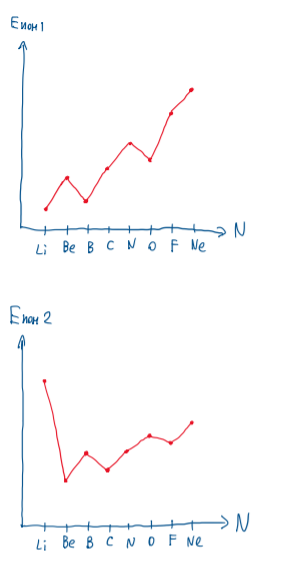
\includegraphics[scale=1.3]{3.png}}
\end{figure}

\textit{График для второй ЭИ напоминает график для первой ЭИ, но со сдвигом на один элемент. Наивысшая ЭИ среди элементов (к примеру, для того же второго периода)
	будет у $Li$, поскольку очень сложно оторвать электрон с внутренней оболочки атома.}

\par\smallskip

\textbf{Электроотрицательность - это способность атома в молекуле
	смещать к себе общие электронные пары, то есть, притягивать к
	себе электроны.}

\par\smallskip

Электроотрицательность по периоду возрастает слева направо, а
сверху вниз по группе падает. Самый электроотрицательный
элемент - фтор.

\begin{center}
	\textbf{Для измерения электроотрицательности существует несколько
		шкал:}
\end{center}


\textbf{По Полингу:} $\Delta E = (X-Y)_{measured} -(X-Y)_{expected}$

\par\smallskip

Эта шкала основана на энергии связи при образовании сложного
вещества из простых.

\par\smallskip

\textbf{По Малликену:} ЭО равна полусумме модулей энергии ионизации и
сродства к электрону (в электрон-вольтах).

\par\smallskip

\textbf{Оллред и Рохов определяют электроотрицательность как
	электростатическую силу, действующую между ядром и
	валентными электронами:}

$$\lambda^{AR}= \frac{3590\cdot z_{eff}}{r^2} + 0.744,$$
	
где $z_{eff}$ - эффективный заряд (с учетом экранирования всеми $\bar{e}$), а  $r$ - ковалентный радиус в пм.

\par\bigskip
\par\bigskip
